\documentclass[11pt]{article}

\usepackage[margin=1in]{geometry}
\usepackage{graphicx}
\usepackage{booktabs}
\usepackage{array}
\usepackage{multirow}
\usepackage{xcolor}
\usepackage{hyperref}
\usepackage[numbers,sort&compress]{natbib}
\usepackage{caption}
\usepackage{subcaption}

\hypersetup{
  colorlinks=true,
  linkcolor=blue!50!black,
  citecolor=blue!50!black,
  urlcolor=blue!50!black
}

\graphicspath{{../figures/}}

\title{AutoTeaKG-Silver: An Uncertainty-Aware Evidence Graph for Tea Functional Activity Literature}
\author{Anonymous Authors}
\date{}

\begin{document}
\maketitle

\begin{abstract}
Tea, tea extracts, and tea-derived components are widely studied for antioxidant, anti-inflammatory, metabolic, cardiovascular, neuroprotective, and gut-microbiota-related activities. However, the evidence is fragmented across tea types, component definitions, processing conditions, model systems, and endpoint labels, making it difficult to compare claims or identify where evidence is strong. We introduce AutoTeaKG-Silver, an automatically generated, provenance-rich, uncertainty-aware evidence graph for tea functional activity literature. The system retrieves PubMed records, converts title/abstract and open full-text methods sections into structured evidence records, normalizes activity and evidence labels, extracts processing and extraction context, and exports a graph in which every edge retains source provenance and uncertainty attributes. In the current KG v3 release, AutoTeaKG-Silver contains 635 evidence records, 1,989 nodes, and 8,195 edges. The pipeline increases processing-context coverage from 146 to 183 records and extraction-context coverage from 154 to 185 records, while explicitly preserving 303 records whose processing or extraction context remains missing. The resulting resource exposes uneven evidence support across activity classes, identifies processing-context reporting gaps, and provides a microbiome-ready graph substrate for downstream mechanism queries. AutoTeaKG-Silver should therefore be interpreted not as a manually verified gold-standard database, but as a reproducible silver-standard evidence infrastructure for living tea bioactivity synthesis.
\end{abstract}

\begin{figure}[t]
  \centering
  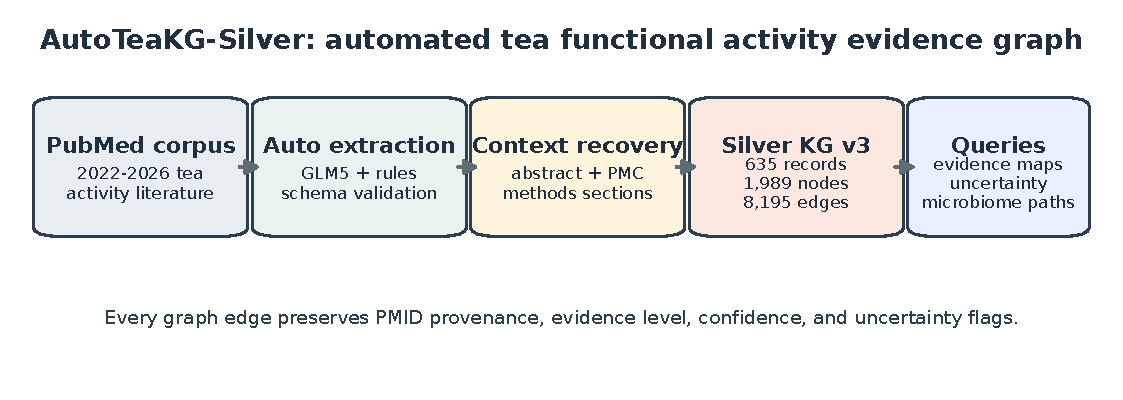
\includegraphics[width=\linewidth]{fig_graphical_abstract.pdf}
  \caption{Graphical overview of AutoTeaKG-Silver. The pipeline converts PubMed tea functional activity literature into structured evidence records, recovers processing and extraction context from abstracts and open PMC methods sections, and exports a provenance-rich uncertainty-aware evidence graph.}
  \label{fig:graphical_abstract}
\end{figure}

\section{Introduction}

Tea is a chemically complex beverage and botanical material with a large literature on potential health-related functions. Reviews have summarized the biological potential of catechins, theaflavins, theanine, caffeine, polysaccharides, and other tea-derived compounds across antioxidant, inflammatory, metabolic, cardiovascular, and neuroprotective endpoints~\cite{luo2024tea_bioactive_review,yang2025bioavailability_tea_polyphenols,rashwan2025tea_polysaccharides_review}. A parallel literature studies how tea processing and extraction alter chemical profiles and product quality~\cite{raghunath2023tea_extraction_review,aaqil2023black_tea_processing_review,wang2024processing_metabolomics}. More recently, tea--microbiome interactions have become a prominent mechanistic theme, especially for metabolic and gut-brain-axis phenotypes~\cite{zhao2024processed_tea_microbiota,song2024oolong_neuroprotection,tian2024obesity_microbiota}. These bodies of work make tea an attractive domain for structured evidence synthesis.

The central difficulty is that tea functional activity evidence is abundant but poorly aligned. A claim about ``green tea'', ``EGCG'', ``tea polyphenols'', ``fermented tea'', or ``tea polysaccharides'' may refer to different materials, processing states, extraction methods, doses, and experimental settings. Evidence strength also varies substantially: animal studies, in vitro experiments, randomized trials, cohort studies, and narrative reviews often appear together in the same prose summary. Narrative reviews are useful for expert interpretation, but they do not provide a machine-readable evidence layer that can answer comparative questions such as which activities have human evidence, which are mostly preclinical, or whether processing information is reported at all.

Existing tea databases do not solve this functional evidence problem. TeaPVs and TeaNekT provide genomic and transcriptomic resources for tea plant biology~\cite{an2022teapvs,zheng2024teanekt}. TRSRD is closer to a tea-domain knowledge graph, but it focuses on risky substances rather than functional activity evidence~\cite{wang2023trsrd}. More general natural-product resources such as NPASS and natural-product drug-interaction knowledge graphs show that natural products can be represented computationally~\cite{zhao2023npass_update,taneja2023npdi_kg}, but they do not encode the tea-specific combination of functional activity, processing context, evidence level, and microbiome mechanism.

We argue that the missing contribution is not another static spreadsheet of tea papers, but an automated evidence infrastructure that makes uncertainty explicit. Manual curation can improve record quality, but it does not scale to a living PubMed-updated resource. Conversely, raw large-language-model extraction is not sufficient unless outputs are constrained by domain schemas, provenance, validation flags, and uncertainty classes. The practical goal is therefore to build a silver-standard graph: a resource that is automatically generated, reproducible, inspectable, and useful for evidence mapping, while avoiding the stronger claim that every edge is expert verified.

This paper introduces AutoTeaKG-Silver, an uncertainty-aware evidence graph for tea functional activity literature. The pipeline retrieves PubMed records, generates structured evidence records, extracts tea type, component group, activity category, study type, evidence level, mechanism labels, microbiome features, and host phenotypes, and then enriches records with processing and extraction context from abstracts and open full-text methods sections. The final graph preserves evidence-record nodes so that each relation can be traced back to a paper, raw claim text, evidence level, and uncertainty flag.

The contributions are fourfold. First, we define a graph-ready evidence model for tea functional activity literature that separates activity claims from study design, evidence level, component context, processing context, and uncertainty. Second, we build an automated silver-standard resource with 635 evidence records and 8,195 graph edges, excluding manual annotation as a data-generation dependency. Third, we show that processing and extraction context remain a measurable bottleneck: targeted extraction improves coverage, but many records lack open full-text or report insufficient methods detail. Fourth, we provide figure-ready query tables and graph outputs that support evidence mapping, processing-aware analysis, and microbiome mechanism exploration.

\section{Materials and Methods}

\subsection{Corpus construction and retrieval archive}

The corpus was constructed from PubMed searches over tea functional activity, component, processing, extraction, microbiome, and human-evidence query blocks. The archived query set covered the publication window from 2022-01-01 to 2026-03-31 and included broad review retrieval, functional activity primary studies, microbiome-focused studies, processing-aware studies, and human evidence searches. Across the larger retrieval batches, records were deduplicated by PMID and normalized into paper-level metadata tables. The manuscript uses the locked auto-only evidence graph derived from these retrievals rather than manually adjudicated mini-gold records.

\subsection{Evidence-record schema}

Each evidence record represents a structured claim anchored to a source paper. Core fields include the source paper identifier, tea type, material form, component group, activity category, endpoint label, study type, evidence level, model system, dose or exposure text, effect direction, mechanism label, microbiota taxon, microbial metabolite, host phenotype, raw claim text, confidence score, and provenance metadata. Activity categories include antioxidant, anti-inflammatory, metabolic improvement, anti-obesity, gut microbiota modulation, neuroprotection, cardiovascular protection, and other. Evidence levels distinguish preclinical in vivo evidence, human observational evidence, human interventional evidence, evidence synthesis, non-quantitative evidence synthesis, and low-preclinical evidence.

\subsection{Auto-only extraction pipeline}

AutoTeaKG-Silver was designed as an auto-only pipeline. The construction path used PubMed metadata, title/abstract text, candidate-record heuristics, GLM5 title/abstract extraction, schema validation, post-processing, duplicate consolidation, and graph export. Manual audit worksheets, mini-gold annotations, and adjudication logs were excluded from the data-generation path. This design choice is deliberate: the goal is to create a scalable silver-standard evidence layer whose uncertainty is visible, rather than to claim expert-level verification for each relation.

\subsection{Processing and extraction context recovery}

Processing and extraction context were recovered in three stages. The first stage used conservative rule-based matching over titles, abstracts, and claim text. The second stage targeted records flagged as missing processing or extraction context and prompted GLM5 to extract only tea-material processing, extraction, and component context from title/abstract text. The third stage queried NCBI E-utilities to map PMIDs to open PMC full text, extracted methods-like sections, and ran a targeted methods-section extractor on records with available full-text context. All targeted extraction steps were patch-first: the model generated a patch table, and patched copies of the silver dataset and KG were regenerated rather than overwriting the base resource.

\subsection{Vocabulary normalization}

LLM surface labels were normalized into a controlled processing and extraction vocabulary. For example, black tea manufacturing and black tea formation were mapped to black tea processing; brick-like form and brick tea processing were mapped to compressed/brick tea processing; cold brewing and hot brewing were mapped to brewing/infusion; and isolation, isolated, and purification were mapped to isolation/purification. Raw LLM labels were retained in mapping tables so that normalization decisions remain auditable.

\subsection{Uncertainty assignment}

Each record was assigned uncertainty flags and an uncertainty class. Flags captured low LLM confidence, missing processing or extraction context, generic mechanism labels, missing named microbiota, taxonomy expansion needs, preclinical-only evidence, review-summary records, uncertain effect direction, and schema validation problems. The uncertainty class summarized these signals into low, moderate, or high uncertainty. This design keeps uncertainty in the graph rather than hiding it during filtering.

\subsection{Graph construction and query tables}

The graph preserves papers and evidence records as explicit nodes. Evidence records are linked to tea type, material form, component group, processing step, extraction method, activity category, study type, evidence level, effect direction, mechanisms, microbiota features, metabolites, host phenotypes, and uncertainty flags. Graph edges retain paper identifier, record identifier, evidence level, study type, effect direction, confidence score, and uncertainty class. Query tables were generated from the final KG v3 to support evidence mapping, activity-by-evidence heatmaps, uncertainty summaries, processing and extraction label distributions, microbiome mechanism subsets, and node/edge composition summaries.

\section{Results}

\subsection{AutoTeaKG-Silver constructs a provenance-rich tea functional activity graph}

The final KG v3 contains 635 silver evidence records, 1,989 nodes, and 8,195 edges (Figure~\ref{fig:kg_composition}). The graph includes paper nodes, evidence-record nodes, activity-category nodes, study-type nodes, evidence-level nodes, tea and component context nodes, processing and extraction context nodes, mechanism nodes, microbiota-feature nodes, microbial-metabolite nodes, host-phenotype nodes, and uncertainty-flag nodes. The explicit EvidenceRecord layer is important because it prevents mechanistic and activity relations from becoming detached from their source papers.

\begin{figure}[t]
  \centering
  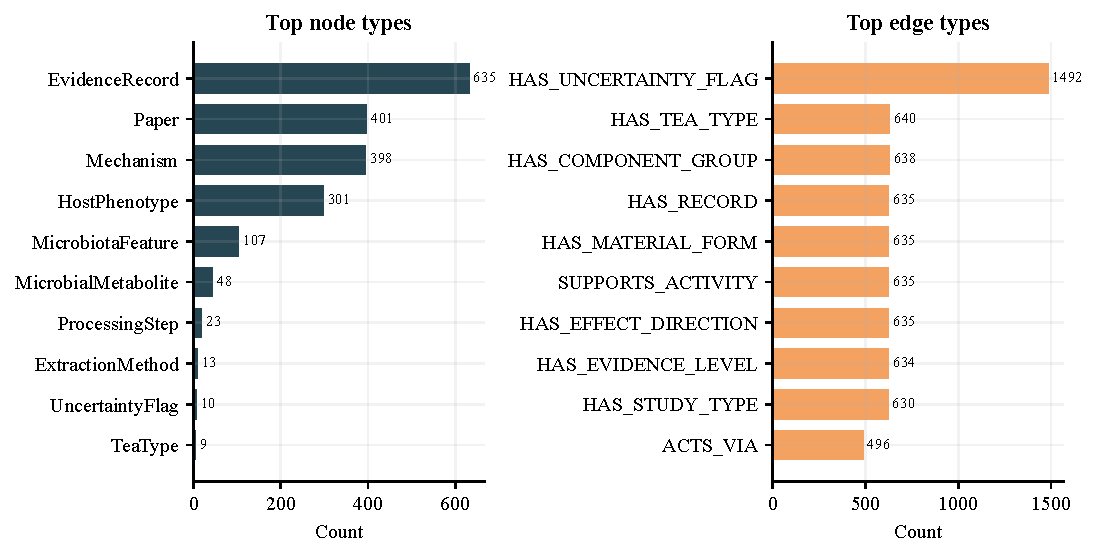
\includegraphics[width=\linewidth]{fig_kg_composition.pdf}
  \caption{Node and edge type composition of KG v3. The graph preserves evidence-record provenance while linking papers, activity categories, evidence levels, tea/component context, processing/extraction context, mechanisms, microbiota features, metabolites, phenotypes, and uncertainty flags.}
  \label{fig:kg_composition}
\end{figure}

\subsection{Evidence-level normalization exposes uneven support across activity classes}

The activity-by-evidence heatmap shows that tea functional activity claims are not evenly supported across evidence levels (Figure~\ref{fig:activity_evidence}). Several activity categories are dominated by preclinical in vivo records and non-quantitative evidence syntheses, while human observational and interventional evidence is concentrated in fewer categories. This pattern supports the central motivation for evidence grading: without evidence-level normalization, review-derived, animal, cohort, and randomized-trial claims are easily mixed into a single apparent evidence base.

\begin{figure}[t]
  \centering
  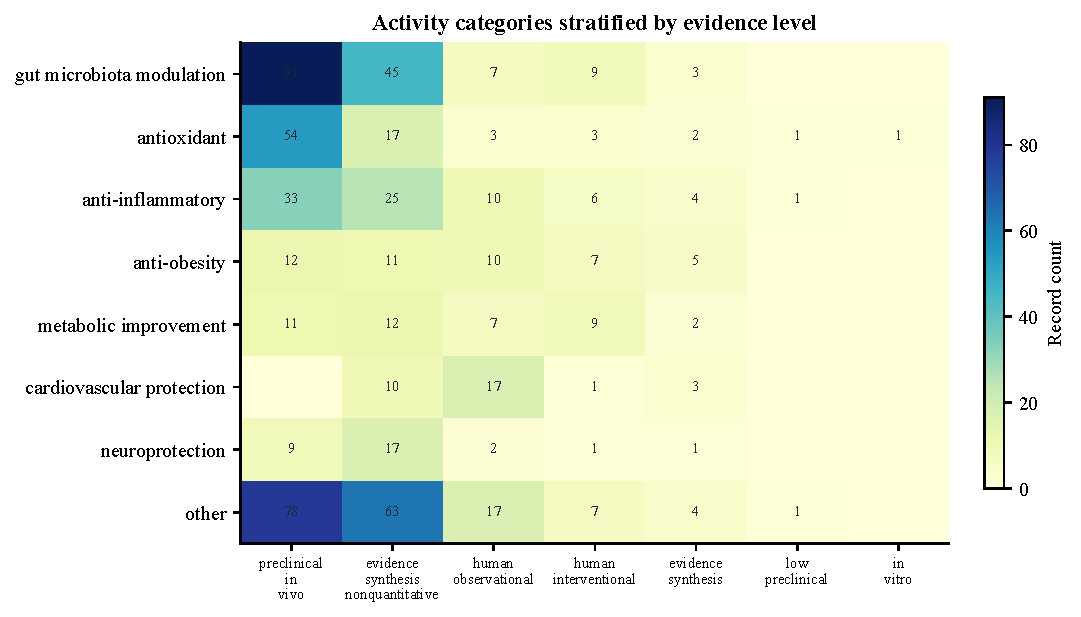
\includegraphics[width=\linewidth]{fig_activity_evidence_heatmap.pdf}
  \caption{Heatmap of normalized activity categories stratified by evidence level in KG v3. The distribution shows that animal evidence and non-quantitative evidence syntheses dominate several activity categories, while human interventional and observational evidence is concentrated in fewer endpoints.}
  \label{fig:activity_evidence}
\end{figure}

\subsection{Targeted extraction improves but does not eliminate missing processing context}

Processing and extraction context increased across extraction stages (Figure~\ref{fig:context_coverage}). Rule-based extraction identified processing context in 146 records and extraction context in 154 records. Abstract-level targeted GLM5 extraction increased coverage, and PMC methods-section extraction further raised processing-context coverage to 183 records and extraction-context coverage to 185 records. The improvement is measurable but modest, indicating that processing context is not uniformly available from abstracts alone.

\begin{figure}[t]
  \centering
  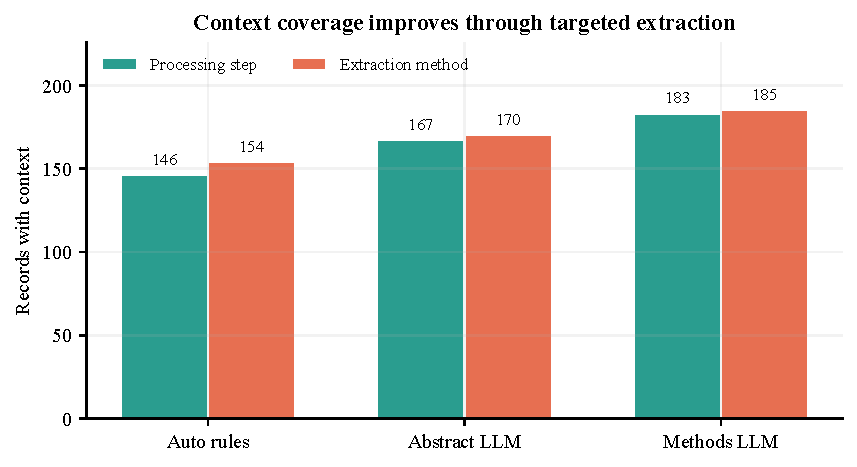
\includegraphics[width=.82\linewidth]{fig_context_coverage.pdf}
  \caption{Context recovery across automated extraction stages. Rule-based extraction established the initial context layer, abstract-level targeted GLM5 extraction added additional context, and PMC methods-section extraction further improved recovery of processing and extraction variables.}
  \label{fig:context_coverage}
\end{figure}

The full-text retrieval analysis clarified why context remains missing. Of 329 records still flagged after abstract-level extraction, 151 records had PMC methods-like sections, while 178 lacked open PMC full text (Figure~\ref{fig:fulltext_funnel}). Methods-section extraction generated patches for all 151 available records and recovered details such as crushing and sieving, cleaning--drying--powdering, steaming and fixation, ultrasonic ethanol extraction, methanol sonication, microwave-assisted extraction, brewing, and isolation/purification.

\begin{figure}[t]
  \centering
  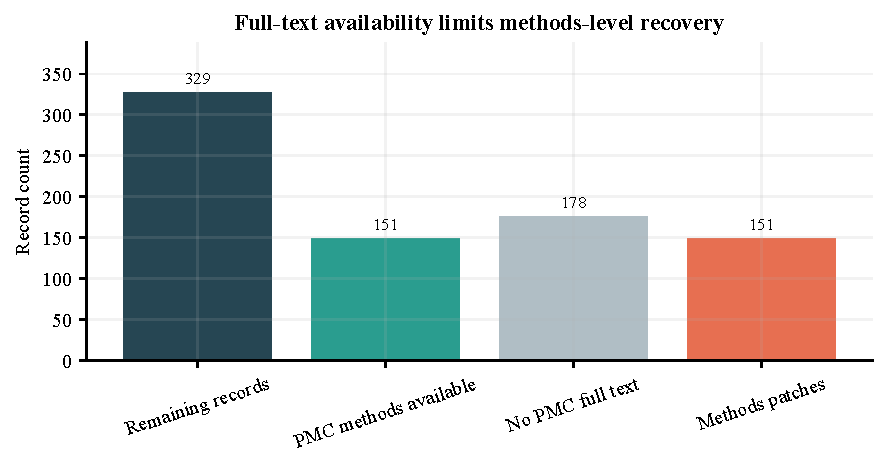
\includegraphics[width=.82\linewidth]{fig_fulltext_methods_funnel.pdf}
  \caption{Full-text methods availability funnel for records that remained missing context after abstract-level extraction. Of 329 remaining records, PMC methods-like sections were available for 151 records, while 178 records lacked open PMC full text.}
  \label{fig:fulltext_funnel}
\end{figure}

\subsection{Vocabulary normalization reduces processing and extraction label fragmentation}

Processing and extraction labels generated by LLM extraction required normalization before graph use. The final vocabulary-normalized KG reduced surface-form fragmentation while retaining raw labels for provenance. Fermentation/oxidation was the dominant processing context, followed by storage/aging, enzymatic treatment, roasting, black tea processing, processing category contrast, drying, steaming/fixation, and crushing/grinding/sieving. Extraction labels were concentrated in other extraction, aqueous extraction, isolation/purification, analytical characterization, brewing/infusion, solvent extraction, ultrasound-assisted extraction, and commercial preparation (Figure~\ref{fig:processing_labels}).

\begin{figure}[t]
  \centering
  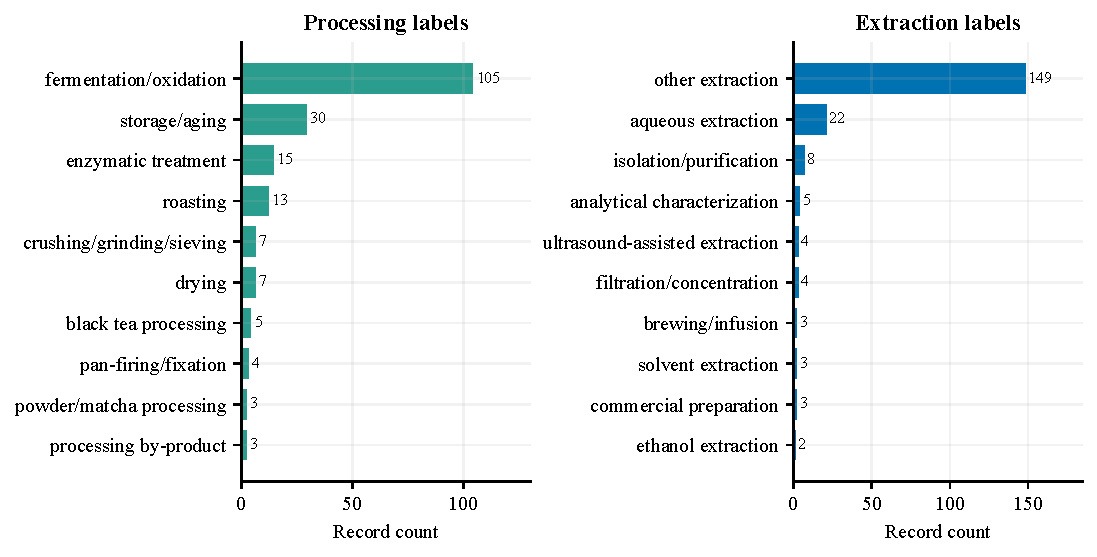
\includegraphics[width=\linewidth]{fig_processing_extraction_labels.pdf}
  \caption{Top normalized processing and extraction labels after abstract-level and methods-section extraction. Vocabulary normalization reduces LLM label fragmentation by mapping surface forms such as black tea manufacturing, matcha production, brewing, isolation, and chromatographic analysis into controlled context labels.}
  \label{fig:processing_labels}
\end{figure}

\subsection{Uncertainty classes make silver-standard status explicit}

The final KG contains 100 low-uncertainty records, 470 moderate-uncertainty records, and 65 high-uncertainty records. The activity-level uncertainty composition (Figure~\ref{fig:uncertainty}) shows that moderate uncertainty dominates the resource. This result is not a defect of the resource; it is the intended operating mode of a silver-standard evidence graph. Instead of filtering uncertainty away, AutoTeaKG-Silver stores uncertainty as a queryable property that downstream users can use to restrict analyses.

\begin{figure}[t]
  \centering
  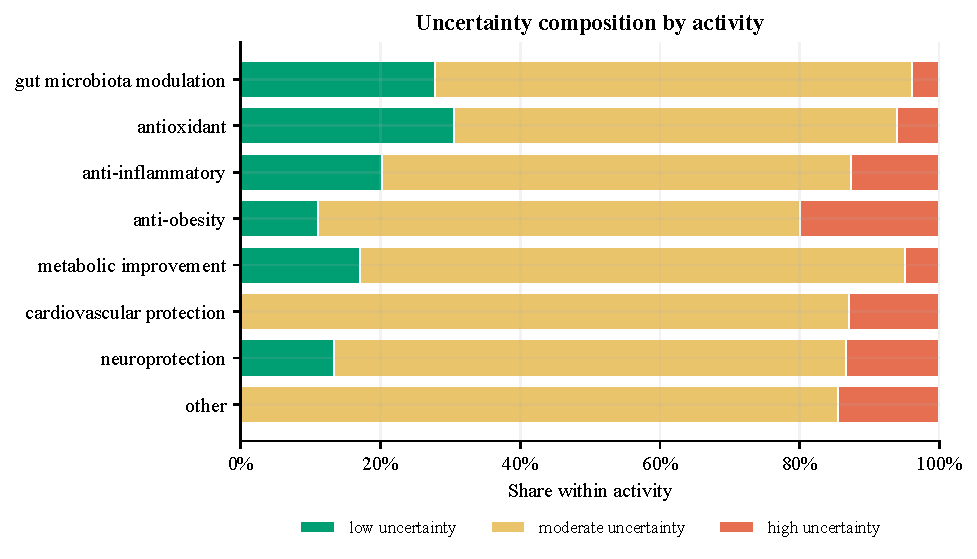
\includegraphics[width=\linewidth]{fig_uncertainty_by_activity.pdf}
  \caption{Uncertainty composition by activity category. Each record was assigned an uncertainty class based on LLM confidence, schema validity, mechanism specificity, context completeness, evidence level, and taxonomy status.}
  \label{fig:uncertainty}
\end{figure}

\subsection{The graph supports microbiome-mechanism queries}

KG v3 contains 190 microbiome-relevant records. These records connect tea types and component groups to gut microbiota modulation, microbial metabolites, host phenotypes, and mechanism labels. The microbiome subset provides a graph-native substrate for querying component--microbiota--metabolite--phenotype paths rather than treating microbiome mentions as isolated keywords. This design is motivated by recent work linking tea polyphenols, oolong tea polyphenols, and tea polysaccharides to microbiota-mediated metabolic, inflammatory, and neuroprotective programs~\cite{zhao2024processed_tea_microbiota,song2024oolong_neuroprotection,tian2024obesity_microbiota,zhang2024fermented_tea_microbiota,arce2025kombucha_rct}.

\section{Discussion}

AutoTeaKG-Silver reframes tea functional activity synthesis as an automated evidence-graph construction problem. The main contribution is not that the system replaces expert review. Rather, the system creates a reproducible and updateable substrate that makes evidence level, provenance, missing context, and uncertainty visible. This framing is important because tea bioactivity claims often differ in study design, material identity, processing state, and mechanism specificity.

The results show that evidence grading changes interpretation. Tea functional activity categories contain a mixture of animal studies, human studies, meta-analyses, randomized trials, and reviews. Treating these records as equivalent would inflate confidence in claims that remain mostly preclinical. By encoding evidence level and study type as first-class graph attributes, AutoTeaKG-Silver allows users to query the evidence base under stricter assumptions.

The processing-context experiments reveal a second challenge. Processing and extraction variables are essential for interpreting tea chemistry and activity, yet many abstracts omit these details. Targeted LLM extraction and PMC methods retrieval improve coverage, but 303 records remain flagged for missing processing or extraction context. This result suggests that future improvements should focus on full-text access and methods-section extraction rather than repeatedly prompting abstracts.

The uncertainty layer is a practical compromise between scale and reliability. A manually curated gold-standard resource would be smaller and slower to update. A raw LLM graph would be larger but difficult to trust. AutoTeaKG-Silver occupies the middle ground: it keeps all records provenance-rich, marks uncertainty explicitly, and provides query tables and figures that can be regenerated from the graph.

\section{Limitations}

This work has four important limitations. First, AutoTeaKG-Silver is a silver-standard resource, not a manually verified gold-standard database. The graph should be used with uncertainty filters when precise biological conclusions are required. Second, the current system relies on PubMed abstracts and open PMC full text; records without PMC full text remain difficult to refine. Third, processing and extraction labels are normalized by rules after LLM extraction, but some labels still represent broad process categories rather than complete experimental protocols. Fourth, the microbiome subgraph includes grouped taxa and generic mechanism labels, so causal interpretation requires additional normalization and full-text validation.

\section{Conclusion}

AutoTeaKG-Silver demonstrates that tea functional activity literature can be converted into an automated, provenance-rich, uncertainty-aware evidence graph. The current KG v3 release contains 635 evidence records, 1,989 nodes, and 8,195 edges, and provides figure-ready query tables for evidence mapping, processing-aware analysis, uncertainty assessment, and microbiome mechanism exploration. The results support a practical conclusion: automated evidence graphs can accelerate tea bioactivity synthesis, provided that uncertainty, provenance, and missing context are treated as first-class data rather than hidden errors.

\bibliographystyle{unsrtnat}
\bibliography{../references/references}

\end{document}
